\chapter{Adaptações e Mudanças}

Neste tópico serão abordadas as mudanças que aconteceram no processo desde a sua validação na entrega 1, tendo também os esclarecimentos sobre o porquê de tais mudanças.

  \textbf{Adicionando o atributo ``Prioridade'' nos casos de uso:} Visto que a solução criada pela equipe de Engenharia de Requisitos possuía um alto número de casos de uso, viu-se que era necessário um modo de criar uma hierarquia de quais eram críticos para o sistema e quais teriam o menor valor agregado para o cliente. Por meio dessa necessidade o time decidiu por adotar o atributo prioridade em seus Casos de Uso para verificar a importância de cada U.C. no software proposto.

  \textbf{Atividade ``Definir Arquitetura'' foi modificada para ``Modelar Diagrama de Caso de Uso'':}
  Tendo como base a antiga atividade no projeto de ``Definição de Arquitetura'' dava-se para ver que a mesma já criava um artefato chamado ``Diagrama de Caso de Uso'', não correspondente exatamente ao que ela era proposta para fazer. Tendo reconhecido tal erro a equipe resolveu renomear a atividade, mas ainda mantendo seus princípios e artefatos criados.

  \textbf{Especificação Suplementar deixou de ser um artefato e agora é incorporado ao Visão:} A atividade já estava sendo feita pois é uma parte que já necessitava estar sido inclusa dentro do Visão, visto a falta de nexo entre o processo e a realidade a equipe resolveu retirar o artefato único de especificação suplementar e apenas deixa-lo na parte de refinar o documento Visão.

  \textbf{A atividade “Priorização requisitos” foi renomeada para ``Priorização de Casos de Uso'' e agora é executada após a atividade ``Modelar Diagrama de Caso de Uso'':} Tal atividade tinha como intuito a parte proposta pela ementa da disciplina na qual a equipe de Engenharia de Software deveria ir até o professor da disciplina para assim partir para a implementação. Tal atividade no processo estava acontecendo antes mesmo da criação do modelo de Caso de Uso o que constituía um erro. Então com a mudança de ``Definir Arquitetura'' para ``Definir Modelo de Caso de Uso'', nada mais correto que tal atividade viesse antes da priorização dos mesmos.

  O processo final de engenharia de requisitos encontra-se na figura \ref{fig:processo}.

  \begin{sidewaysfigure}
    \begin{figure}[H]
      \centering
      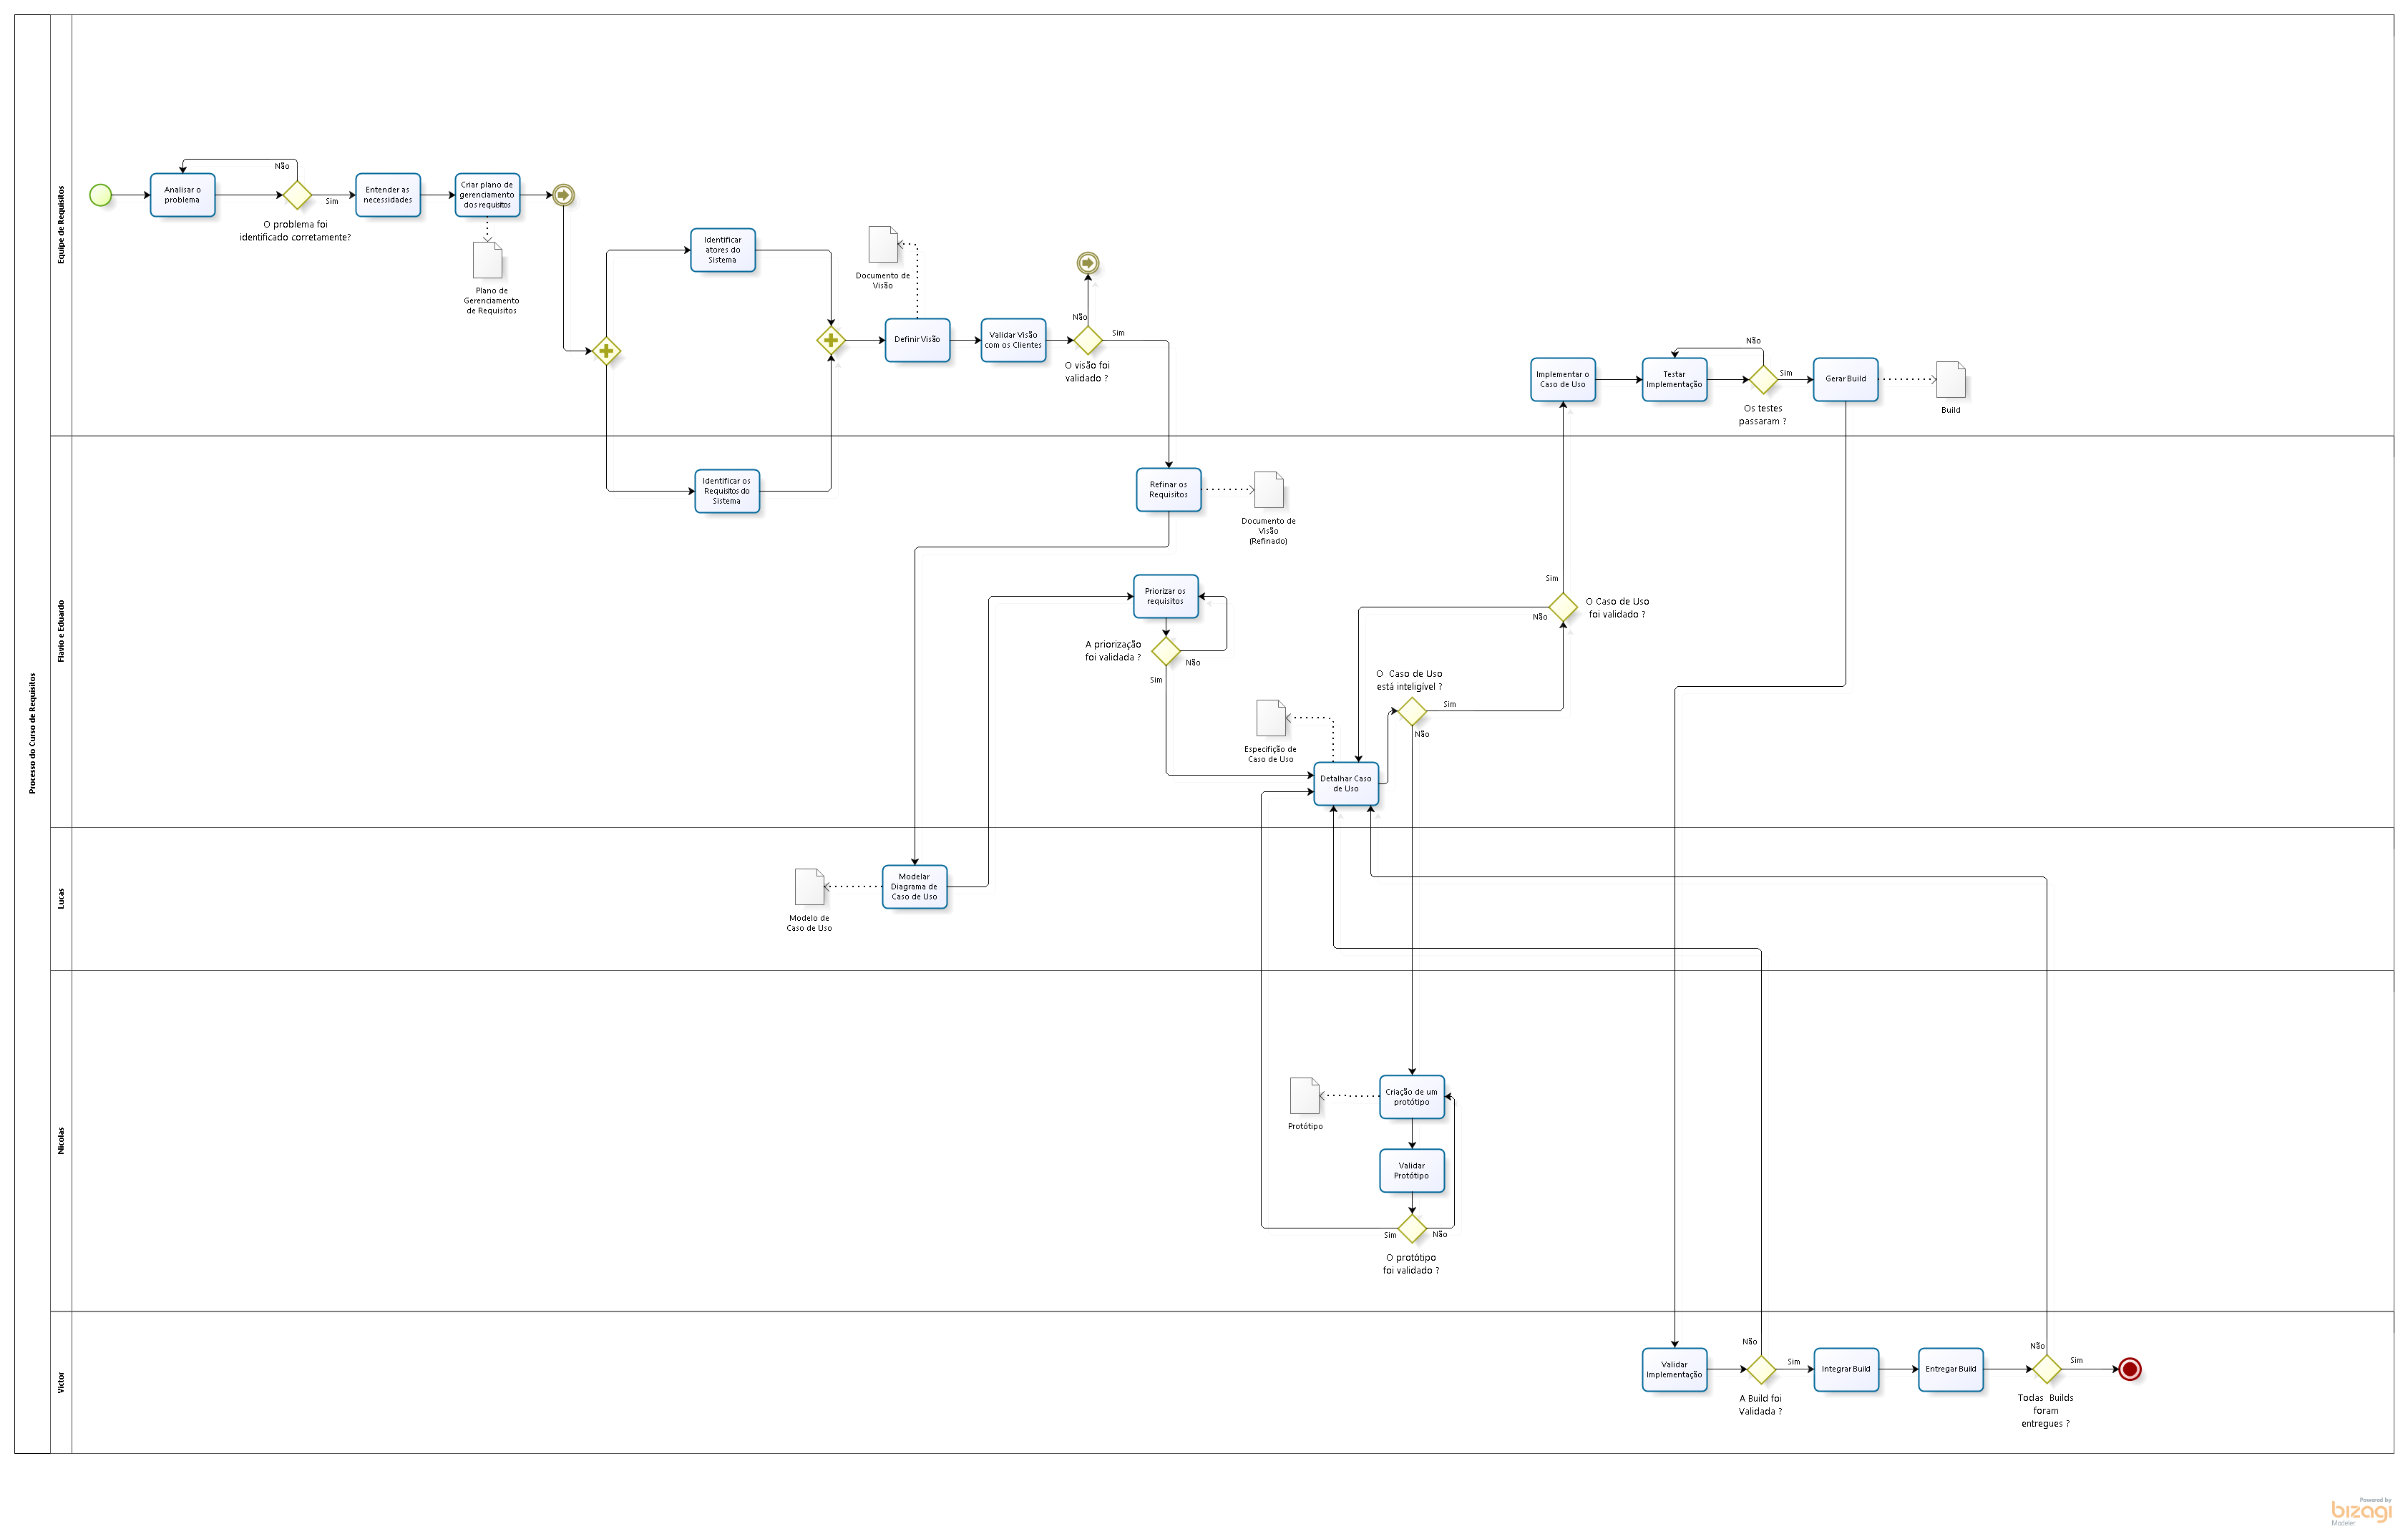
\includegraphics[width=0.95\textwidth]{figuras/ModeloV5}
      \caption{Processo de Engenharia de Requisitos}
      \label{fig:processo}
    \end{figure}
  \end{sidewaysfigure}
  \clearpage
